%%%%%%%%%%%%%%%%%%%%%%%%%%%%%%%%%%%%%%%%%%%%%%%%%%%%%%%%%%%%%%%%%%%%%%%%
% PACKAGES
%%%%%%%%%%%%%%%%%%%%%%%%%%%%%%%%%%%%%%%%%%%%%%%%%%%%%%%%%%%%%%%%%%%%%%%%

\documentclass[11pt,a4paper]{article}
\usepackage[czech]{babel}
\usepackage[utf8]{inputenc}
\usepackage[T1]{fontenc}
\usepackage{lmodern}
\usepackage{textcomp}
\usepackage{geometry}
\usepackage[hidelinks]{hyperref}
\usepackage{bookmark}
\usepackage{enumitem}
\usepackage{parskip}
\usepackage{titlesec}
\usepackage{graphicx}
\usepackage{float}
\usepackage{tabularx,array}
\usepackage{booktabs} 
\usepackage{comment}
\usepackage{siunitx}
\usepackage{threeparttable}
\usepackage[format=hang]{caption}

\geometry{margin=2.2cm}
\setlist{nosep,leftmargin=2em}

%%%%%%%%%%%%%%%%%%%%%%%%%%%%%%%%%%%%%%%%%%%%%%%%%%%%%%%%%%%%%%%%%%%%%%%%
% COMMANDS CONFIG
%%%%%%%%%%%%%%%%%%%%%%%%%%%%%%%%%%%%%%%%%%%%%%%%%%%%%%%%%%%%%%%%%%%%%%%%

% Definice subsubsubsection
\titleclass{\subsubsubsection}{straight}[\subsubsection]
\newcounter{subsubsubsection}[subsubsection]
\renewcommand\thesubsubsubsection{\thesubsubsection.\arabic{subsubsubsection}}
\titleformat{\subsubsubsection}
  {\normalfont\normalsize\bfseries}{\thesubsubsubsection}{1em}{}
\titlespacing*{\subsubsubsection}{0pt}{1.25ex plus 1ex minus .2ex}{0.75ex plus .2ex}

% Definice subsubsubsubsection
\titleclass{\subsubsubsubsection}{straight}[\subsubsubsection]
\titleformat{\subsubsubsubsection}
  {\normalfont\normalsize\bfseries}{}{0pt}{}%
\titlespacing*{\subsubsubsubsection}
  {0pt}{1.25ex plus 1ex minus .2ex}{0pt}

% Nastavení hloubky číslování a obsahu
\setcounter{secnumdepth}{4} % Hloubka číslování
\setcounter{tocdepth}{4}    % Hloubka obsahu

% Přidání subsubsubsection do obsahu
\makeatletter
    \newcommand{\l@subsubsubsection}{\@dottedtocline{4}{7em}{4em}}
    % subsubsubsubsection z obsahu úplně vyhodíme (i kdyby bylo něco v .toc)
    \newcommand*\l@subsubsubsubsection[2]{}
    
    % Mapování úrovní pro správné záložky
    \providecommand*{\toclevel@subsubsubsection}{4}
    \providecommand*{\toclevel@subsubsubsubsection}{5}
\makeatother

% Zalamování v tabulkách
\newcolumntype{L}{>{\raggedright\arraybackslash}X}
\newcolumntype{P}{>{\ttfamily\raggedright\arraybackslash}X} 


%%%%%%%%%%%%%%%%%%%%%%%%%%%%%%%%%%%%%%%%%%%%%%%%%%%%%%%%%%%%%%%%%%%%%%%%
% DOCUMENT START
%%%%%%%%%%%%%%%%%%%%%%%%%%%%%%%%%%%%%%%%%%%%%%%%%%%%%%%%%%%%%%%%%%%%%%%%

\begin{document}

%%%%%%%%%%%%%
% Title page
%%%%%%%%%%%%%

\begin{titlepage}
\begin{center}
    \Huge{\textsc{Vysoké učení technické v~Brně}}\\
    \vspace{0.5em}
    \huge{\textsc{Fakulta informačních technologií}}\\
    \vspace{\stretch{0.382}}
    {{\Huge Simulační studie\\}
     \vspace{0.6em}
     {\huge Hledání úzkých míst v~řetězci pěstování ozimé pšenice\\}
     \vspace{0.3em}
     {\Large Modelování a simulace (IMS): T3 -- SHO Model výroby v~oblasti zemědělství\\}}
    \vspace{\stretch{0.618}}
\end{center}
\begin{flushright}
Jan Kalina (\texttt{xkalinj00})
\end{flushright}
\vspace{-0.5\baselineskip}
\noindent
2025
\hfill
David Krejčí (\texttt{xkrejcd00})
\end{titlepage}

\newpage


%%%%%%%%%%%%%%%%%%%%
% Table of contents
%%%%%%%%%%%%%%%%%%%%

{
    \hypersetup{linkcolor=black}
    \tableofcontents
}

\newpage


%%%%%%%%%%%%%%%%%%%%%%%%%%%%%%%%%%%%
% Introduction and Conceptual model
%%%%%%%%%%%%%%%%%%%%%%%%%%%%%%%%%%%%

\section{Úvod}

Tato simulační studie se zabývá tvorbou konceptuálního a simulačního modelu podzimního setí ozimé pšenice zemědělským podnikem a následnou simulací jeho chování v~čase a vyhodnocením provedených experimentů. Model reprezentuje klíčové operace výrobního procesu (zpracování půdy, hnojení, setí, dokončovací práce) a jejich vzájemné vazby v~prostředí omezených zdrojů, proměnlivého počasí a nenulové poruchovosti techniky.

Pro středně velké zemědělské farmy v~České republice (řádově stovky hektarů orné půdy) představuje správné načasování a organizace setí ozimé pšenice klíčový úkol z~hlediska zajištění výnosu a efektivity provozu. Včasné zasetí v~optimálním agrotechnickém termínu (obvykle od druhé poloviny září do poloviny října) je zásadní pro dobré přezimování a výnos plodiny. Na středně velkých farmách však vzniká otázka, zda dostupné zdroje (technika a pracovní síla) dovolí zasít veškerou výměru pšenice v~požadovaném čase, a jaké faktory mohou způsobit zpoždění. V~praxi je totiž velmi obtížné zvládnout zasít kompletní plochu ozimé pšenice v~optimálním termínu -- limitujícími faktory bývají omezené kapacity strojů a pracovníků i nepříznivé počasí. Tyto problémy se projevují zvláště u~farem s~větším osevním plánem ozimů.

Pomocí simulačních běhů a systematicky navržených experimentů je možné porovnat různé varianty organizace práce a technického vybavení bez zásahu do skutečného provozu. Tím lze předem odhadnout dopady změn (např. přidání stroje, prodloužení směn, změny technologie zpracování půdy) na včasnost setí a potenciální ztráty výnosu a na tomto základě formulovat doporučení pro úpravu reálného systému.

\subsection{Počáteční otázka}

Hlavní otázkou, kterou se studie zabývá, je \emph{Kde se v~řetězci pěstování ozimé pšenice na průměrně velké až větší farmě v~ČR nacházejí kritická úzká místa a jaké změny v~konfiguraci technologické linky je nutné provést pro minimalizaci prostojů a bezpečné dodržení agrotechnického termínu?}.

V~této simulační studii bude zodpovězeno také  několik dalších souvisejících otázek jako např. \emph{Který kritický technologický krok nebo zdroj (stroj, pracovník, \dots) vykazuje v~simulovaném modelu nejnižší průchodnost a nejvyšší míru využití, čímž se stává hlavním úzkým hrdlem výrobní linky?} nebo \emph{Jak velký dopad by mělo nasazení dalšího secího stroje nebo prodloužení směny pracovníků?}. V~neposlední řadě studie analyzuje, jaký je pravděpodobnostní dopad vlivu stochastických událostí (např. výpadek secího stroje, změna počasí) na včasnost dokončení setí a jak se toto riziko promítne do ekonomické efektivity provozu a následného výdělku.
\subsection{Zdroje faktů}

Pro konstrukci modelů byly nejprve shromážděny konkrétní údaje z~odborných zdrojů, které tvoří faktickou základnu modelovaného problému -- využita byla například na státní úrovni verifikovaná data z~\href{https://csu.gov.cz/}{\emph{Českého statistického úřadu}} nebo profesionální data ze známých agronomických magazínů jako je \href{https://www.agromanual.cz/}{\emph{Agromanuál.cz}}. Jedná se o~kvantitativní i kvalitativní data charakterizující pěstování ozimé pšenice, mechanizaci setí a klimatické podmínky během podzimních prací a další, pro naši studii nezbytná, data (viz kapitola \ref{sec:rozbor-tematu}).

Konceptuální model a vstupní parametry byly verifikovány z~hlediska souladu s~realitou několika způsoby. Zdroje pro tatáž data byla křížově porovnána -- např. při výběru vhodných referenčních zemědělských strojů byly jejich výkonové charakteristiky uvedené na internetových obchodech srovnány s~údaji od výrobců a celkově byly vybírány takové stroje, které mají průměrný výkon (tj. výkon typický pro stroj dané kategorie).

Dalším významným zdrojem dat, jakožto podkladů pro hypotézy, byla osobní zkušenost jednoho z~autorů této studie, Jana Kaliny, který v~průběhu tří let strávil 6 měsíců prací v~zemědělském podniku I.MTZ s.r.o.\cite{imtz} v~Sušicích u~Moravské Třebové.

\section{Použité metody a technologie}

Studie zpracovává postup tvorby konceptuálního a simulačního modelu a následné simulace podle metodiky předmětu \emph{Modelování a simulace} (IMS)\cite{ims} na Fakultě informačních technologií Vysokého učení technického v~Brně. 

Konceptuální model byl zpracován ve webové aplikaci \texttt{draw.io}\cite{draw.io}, která je světově nejpoužívanější webovou aplikací určenou ke tvorbě diagramů, a to ve formě Petriho sítě (bližší popis naleznete v~kapitole \ref{forma-konceptualniho-modelu}).

Samotná simulace byla provedena pomocí diskrétního simulačního modelu tohoto systému hromadné obsluhy (SHO) implementovaného v~jazyce \texttt{C++} za využití nejnovější verze knihovny \texttt{SIMLIB/C++} 3.09\cite{simlib}. Simulátor byl navržen pro systém GNU Linux a testován na operačním systému Ubuntu 24.04.3 LTS (návod k~překladu a spuštění viz kapitola \ref{jak-spustit-simulacni-model})

\section{Rozbor tématu -- Pěstování ozimé pšenice}\label{sec:rozbor-tematu}

\subsection{Osevní plocha}

Podzimní setí ozimé pšenice představuje klíčovou operaci v~rostlinné výrobě, která má přímý dopad na výnos následující sklizně. Ozimá pšenice představuje dlouhodobě nejpěstovanější plodinu v~České republice s~osevní plochou pohybující se v~posledních letech kolem 750 tisíc hektarů\cite{čsú-plocha-pšenice}, což odpovídá přibližně 30~\% celkové osevní plochy v~zemi\cite{čsú-plocha-celkově}. Průměrné výnosy ozimé pšenice dosahují zhruba 6 tun zrna na hektar\cite{agromanuál-výnos-tun-na-hektar}, což při uvedené výměře znamená celkovou produkci okolo 4,8 milionu tun zrna ročně. 

Farmy v~ČR dosahují průměrné velikosti kolem 120~ha\cite{zsčr-zpráva}, což je v~evropském kontextu nadprůměrná hodnota, a umožňuje rozsáhlé polní operace s~využitím moderní mechanizace. Naše simulační studie se zaměřuje na farmu o~rozloze 200~ha, tedy větší než průměrná, kde se plánuje pěstovat ozimou pšenici na celé výměře. % TODO: zeptat se na rozlohu farmy

\subsection{Technologická linka pěstování ozimé pšenice}\label{technologicka-linka-pestovani-ozime-psenice}

Samotný proces pěstování ozimé pšenice lze rozdělit do několika na sebe navazujících operací. Nejprve musí dojít ke sklizni předplodin. Po sklizni předplodiny následuje posečení a úklid posklizňových zbytků (strniště, sláma). Běžnou praxí je provést brzy po sklizni předplodiny mělkou podmítku (do \textasciitilde15 cm)\cite{eos-pěstování-pšenice-ozimé} talířovým či radličkovým podmítačem nebo kypřičem, aby se podpořilo klíčení výdrolu a plevelů a částečně zapravily zbytky. Tato operace zvaná \uv{podmítka} šetří vláhu a čas pro následné práce tím, že podporuje rozklad organických zbytků a ničí plevel v~povrchové vrstvě půdy. Následuje základní zpracování půdy pro setí pšenice. Tradiční metodou je orba klasickým pluhem na podzim (do hloubky \textasciitilde20--22 cm)\cite{agkaizen-pšenice-ozimá}, po níž před setím ještě musí proběhnout předseťová příprava (např. projíždění kompaktorem) za účelem rozmělnění hrud a urovnání povrchu. 

Alternativou je metoda \uv{min-till} (\emph{minimum tillage} čili \emph{minimální orba, redukované obdělávání}), při které je půda zpracována pouze mělkým kypřením (talířovým či radličkovým podmítačem nebo kypřičem) do hloubky kolem 10--15~cm a následně se seje přímo do takto zpracovaného pole\cite{agromanuál-klasika-vs-min-till}. Redukované obdělávání půdy tak nejen snižuje narušení půdy způsobené klasickou orbou, ale také zmírňuje náklady na pořízení těžkých strojů pro klasickou orbu, palivo, čas a potřebné lidské zdroje\cite{kuhn-min-till}. Moderní secí stroje navíc často umožňují kombinované operace, kdy při setí zároveň půdu mělce zkypří a utuží, takže odpadá zvláštní předseťová příprava\cite{pöttinger-efektivní-výroba}.

Po přípravě půdy následuje nejdůležitější činnost z~celé technologické linky pěstování pšenice ozimé, kterou je setba (ta bude podrobněji probrána později). Po dokončení setby musíme ještě provést závěrečné zaválení pomocí kultivačního válce, čímž dojde k~zapravení zrna do půdy a vytvoření ochranné vrstvy.

\subsection{Agrotechnické okno pro setí ozimé pšenice}\label{agrotechnicke-okno}

Ozimá pšenice se v~českých podmínkách vysévá zpravidla od druhé poloviny září do poloviny října, přičemž optimální agrotechnický termín setí pro většinu odrůd je přibližně od 20. září do 15. října\cite{wikifarmer-kdy-pěstovat}. Důvodem je potřeba, aby rostliny stihly dostatečně vzejít a odnožit před zimou, což zvyšuje šanci dobrého přezimování a na jaře umožňuje vytvořit dostatek klasů pro vysoký výnos. Při časném setí (v~polovině září) mohou některé moderní odrůdy dokonce dosáhnout vyšších výnosů díky prodloužení podzimní vegetace\cite{úroda-časné-setí}, avšak příliš rané setí nese i rizika (přerůstání porostu, podpora chorob a škůdců)\cite{úroda-časné-setí}. Naopak pozdní setí po optimálním termínu obecně pšenici nevyhovuje -- zkrácení podzimní fáze vede k~nedostatečnému odnožení a mělčímu kořenovému systému, což se obvykle promítá do snížení výnosu. Odhaduje se, že každý den zpoždění výsevu znamená přibližný pokles výnosu o~1~\%\cite{mdpi-pozdní-setí}.

V~naší studii se budeme zabývat nejběžnějším oknem pro setí, tedy již zmíněným oknem od 20. září do 15. října\cite{wikifarmer-kdy-pěstovat}.

\subsection{Výkonnost a kapacity strojů}

Zvolení konkrétních typů strojů pro účely našich modelů bylo nezbytné pro co nejpřesnější kvantifikaci výkonu jednotlivých technologických operací, které v~modelech hrají klíčovou roli. Cílem bylo vybrat takové referenční stroje, jejichž technické parametry odpovídají běžné praxi na středně velkých zemědělských farmách v~České republice. Nešlo nám o~jejich teoretickou maximální výkonnost nebo katalogové hodnoty, ale o~realistické hodnoty dosažitelné v~provozních podmínkách. Výběr zahrnoval jak základní pracovní stroje (např. podmítač, pluh, secí stroj), tak i podpůrné prostředky (např. kultivační válec), přičemž jsme se opírali o~kombinaci údajů od výrobců, nabídky českých e-shopů zabývajících se prodejem zemědělských strojů (zejména pak o~e-shop \emph{\href{https://www.eshop-zemedelske-potreby.cz/}{Zemědělské potřeby M+S s.r.o.}} a portál inzercí \emph{\href{https://www.agriaffaires.cz/}{Agriaffaires}}) a vlastních zkušeností. 

Součástí tohoto postupu bylo také stanovení tzv. efektivní plošné výkonnosti (EFC), která zohledňuje nejen pracovní záběr a rychlost stroje, ale i ztráty způsobené otáčením, seřizováním, doplňováním materiálu přejezdy apod. (blíže viz kapitola \ref{popis-konceptualniho-modelu}).

\begin{table}[H]
    \centering
    \begin{threeparttable}
        \setlength{\tabcolsep}{4pt}
        \renewcommand{\arraystretch}{1.12}
        \small
        \begin{tabularx}{\linewidth}{@{}lXrccc@{}}
            \toprule
            Kategorie & Model & \textasciitilde{Cena} [Kč] & Kapacita & $W$ [m] & $S$ [km/h] \\ \midrule
            Podmítací stroj & ROL EX Gruber APG 3.0\cite{eshop-zp-podmítač}
              & 200\,000 & -- & 3 & 6--12 \\
            Pluh & AGROPA AGN21-440\cite{eshop-zp-pluh}
              & 300\,000 & -- & 1,8 & 5--7 \\
            Kombinátor & Campbell ROL EX WFC 3.0\cite{eshop-zp-kombinátor}
              & 150\,000 & -- & 3 & 4--12 \\
            Kombinovaný mělký kypřič & Finisher 400\cite{eshop-fomex-kombinovaný-kypřič}
              & 1\,750\,000 & -- & 4.15 & 8--14 \\
            Rozmetadlo hnoje & Cynkomet N-221/3-3 CS LINE 6\cite{eshop-zp-rozmetadlo-hnoje}
              & 700\,000 & 6 t & 7 & 6--12 \\
            Secí stroj & Unia Polonez 550/3D\cite{eshop-zp-secí-stroj}
              & 500\,000 & 550 l & 3 & 5--9 \\
            Kultivační válec & Cambridge ROL EX WPH 4.5\cite{eshop-zp-kultivační-válec}
              & 300\,000 & -- & 4,5 & 4,5--7,5 \\
            \bottomrule
        \end{tabularx}
        \begin{tablenotes}[flushleft]
            \footnotesize
            \item Pozn.: $W$ je pracovní záběr, $S$ je doporučený rozsah pracovní rychlosti.
        \end{tablenotes}
    \end{threeparttable}
    \caption{Souhrn parametrů vybraných zemědělských strojů.}
    \label{tab:shrnuti-stroju}
\end{table}

\subsection{Organizace pracovníků na farmě}

Organizačně farma disponuje omezeným počtem pracovníků, traktorů a zemědělských strojů. Z~osobních zkušeností jde často o~rodinný podnik, kde se o~veškerou polní práci stará pouze několik stálých pracovníků a v~době vrcholících podzimních prací (setí ozimů, sklizeň kukuřice, orbová příprava na jaro) farmy často najímají sezónní výpomoc nebo pracují prodloužené směny, aby vše stihly včas -- v~období setí ozimů je běžné pracovat směny o~délce 10, někdy i 12, hodin.

\subsection{Ekonomická analýza produkce}\label{sec:ekonomika}

Pro validitu simulačního modelu je nezbytné, aby vstupní ekonomické parametry odpovídaly tržní realitě a detailní struktuře nákladů moderní agrotechniky. Ekonomika pěstování ozimé pšenice je v~modelu tvořena součtem variabilních nákladů (osivo, základní hnojení, kvalitativní přihnojení, chemická ochrana), provozních nákladů (stroje, lidská práce) a výnosovou stránkou. V~rámci našeho modelu pracujeme s~cenovou hladinou a technologickými postupy odpovídajícími hospodářskému roku 2024/2025.

\subsubsection{Přímé materiálové náklady}\label{materialove-naklady}

Nejvýznamnější položkou v~rozpočtu pěstitele jsou náklady na materiál, které byly pro účely přesnější simulace rozděleny do čtyř klíčových kategorií. Toto rozdělení umožňuje lépe simulovat dopad intenzifikace výroby na konečný výnos.

\begin{itemize}
    \item \textbf{Osivo:} Pro založení porostu uvažujeme náklady na certifikované osivo ve výši \textbf{2\,200 Kč/ha}. Tato částka odpovídá výsevu cca 180--200 kg/ha při použití mořeného osiva kategorie C1\cite{agromanuál-ceny-osiv}.
    
    \item \textbf{Hnojení a výživa:} Model rozlišuje mezi základním hnojením a dodatečnou výživou. 
    \begin{itemize}
        \item \textit{Základní hnojení:} Aplikace před setím nebo v~raných fázích (NPK, základní dusík) je stanovena na \textbf{3\,500 Kč/ha}\cite{agromanuál-hnojiva-2024}.
        \item \textit{Produkční přihnojení} Pro dosažení vyššího výnosu a kvality zrna (objemová hmotnost, lepek) model počítá s~nákladem \textbf{3\,000 Kč/ha} na jarní a kvalitativní přihnojení dusíkatými hnojivy.
    \end{itemize}

    \item \textbf{Chemická ochrana rostlin:} Pro udržení zdravotního stavu porostu (ochrana proti plevelům, chorobám a škůdcům) a regulaci růstu je vyhrazena částka \textbf{6\,000 Kč/ha}\cite{úze-nákladovost-pšenice}. Tato hodnota reflektuje intenzivní technologii pěstování nutnou pro dosažení výnosů nad 6 tun.
\end{itemize}

\noindent \textit{Celkové materiálové náklady na hektar tedy v~modelu činí 14\,700 Kč.}

\subsubsection{Náklady na mechanizaci a lidskou práci}

Další skupinu tvoří náklady spojené s~provozem techniky a odměňováním pracovníků. Tyto parametry vstupují do simulace jako hodinové sazby a jsou přepočítávány dle reálného času operací.

\begin{itemize}
    \item \textbf{Provoz traktoru:} Hodinová sazba traktoru je stanovena na \textbf{900 Kč/h}. Tato částka pokrývá variabilní náklady, primárně spotřebu motorové nafty a běžnou údržbu stroje, bez započtení plné účetní amortizace\cite{mechanizace-zemědělství-kalkulace}.
    
    \item \textbf{Cena práce:} Náklad na operátora stroje je v~modelu nastaven na \textbf{250 Kč/h}. Tato hodnota představuje optimalizovaný mzdový náklad (např. při využití sezónních pracovníků nebo nižším zdanění v~rámci rodinných farem) a je nižší než celostátní průměr superhrubé mzdy\cite{platy-cz-traktorista}.
\end{itemize}

\subsubsection{Výnosy a výsledná bilance}

Výnosová stránka modelu je definována očekávanou sklizní a tržní realizační cenou. Díky intenzivnějšímu vstupu hnojiv a ochrany (viz sekce \ref{materialove-naklady}) počítá model se zvýšeným průměrným výnosem \textbf{6,5 t/ha}. Při fixované realizační ceně \textbf{4\,800 Kč/t} (odpovídající průměru cen 2024/2025) generuje jeden hektar tržby ve výši 31\,200 Kč\cite{szif-komoditni-zprava}.

V~Tabulce \ref{tab:ekonomika-ha} je uveden souhrnný přehled kalkulace na 1 hektar dle aktuálních parametrů simulace.

\begin{table}[H]
    \centering
    \begin{threeparttable}
        \setlength{\tabcolsep}{6pt}
        \renewcommand{\arraystretch}{1.2}
        \small
        \begin{tabularx}{\linewidth}{@{}Xr@{}}
            \toprule
            Položka & Hodnota [Kč/ha] \\ \midrule
            \textbf{Příjmy celkem} (6,5 t/ha $\times$ 4 800 Kč/t) & \textbf{31\,200} \\
            \midrule
            Osivo & 2\,200 \\
            Základní hnojení & 3\,500 \\
            Dodatečný dusík (přihnojení) & 3\,000 \\
            Chemická ochrana (postřiky) & 6\,000 \\
            Strojní náklady (odhad dle přejezdů)\tnote{1} & 4\,500 \\
            Lidská práce (mzdy -- odhad dle přejezdů)\tnote{1} & 1\,250 \\
            \textbf{Náklady celkem} & \textbf{20\,450} \\
            \midrule
            \textbf{Hrubý zisk (před zdaněním a pachtovným)} & \textbf{10\,750} \\
            \bottomrule
        \end{tabularx}
        \begin{tablenotes}[flushleft]
            \footnotesize
            \item[1] Hodnoty strojních nákladů a práce jsou odvozeny z~průměrného počtu přejezdů (cca 5 Mth/ha) při sazbách 900 Kč/h (stroj) a 250 Kč/h (práce).
        \end{tablenotes}
    \end{threeparttable}
    \caption{Kalkulace hrubé marže pěstování pšenice na 1 hektar.}
    \label{tab:ekonomika-ha}
\end{table}

\section{Koncepce}

\subsection{Popis konceptuálního modelu}\label{popis-konceptualniho-modelu}

Modelová farma je středně velký až větší zemědělský podnik zaměřený na polní rostlinnou výrobu. Hospodaří na výměře přibližně 200~ha orné půdy, na níž pěstuje zejména obilniny (pšenici ozimou, ječmen, \dots) a olejniny (řepku, řepku ozimou). Pšenice ozimá představuje hlavní plodinu, která zabírá významnou část modelové farmy a tvoří její hlavní zisk. Farma disponuje odpovídajícím strojovým vybavením pro zpracování půdy a setí a zaměstnává několik kvalifikovaných pracovníků. Tito pracovníci společně zajišťují veškeré polní operace v~průběhu sezóny a technickou správu traktorů a ostatních strojů. Organizačně farma funguje v~konvenčním režimu, avšak zvažuje i zavádění minimalizovaných postupů zpracování půdy s~cílem zvýšit efektivitu (zavedení \uv{min-till}\cite{kuhn-min-till}).

Délka trvání jednotlivých operací na jednom poli je odvozena z~výpočtu efektivní plošné výkonnosti konkrétních referenčních strojů (viz kapitola \ref{charakteristiky-stroju}), přičemž efektivní plošná výkonnost EFC je spočtena z~jejich pracovního záběru $W$, rychlosti práce $S$ a vhodně zvoleného koeficientu polní efektivity $\eta$.

Systém je zatížen omezenými zdroji a stochastickými vlivy. K~dispozici jsou dva traktory a univerzální sada v~kapitole \ref{charakteristiky-stroju} uvedených strojů, přičemž každý konkrétní stroj může být v~daném okamžiku obsluhován pouze jedním traktorem. Počet pracovníků je ve výchozím stavu modelu ztotožněn s~počtem traktorů. Každý pracovník (univerzální pracovník -- umí řídit traktor, provádět opravy apod.) má přidělenou směnu délky 10--12 hodin a po skončení směny musí odejít na odpočinek (po dobu $24\text{ hod.}-T_{směna}$), přičemž rozpracovaná operace na poli může zůstat nedokončená a pokračuje se v~ní následující \uv{pracovní} den.

Dostupnost práce na poli je dále omezena počasím -- každý den v~období září--říjen je v~modelu označen jako \uv{pracovní} nebo \uv{nepracovní} s~danou pravděpodobností (např. $0,4$)\cite{workable-days}. Pokud je daný den z~důvodu počasí \uv{nepracovní}, tak po celý tento den žádný pracovník s~traktorem nevyjede na pole, protože pro to nejsou příznivé meteorologické a půdní podmínky. Tato koncepce je dále popsána v~kapitole \ref{workable-days}.

V~případě, že je den \uv{pracovní}, tak se traktor na pole pokusí vyjet, ale to pouze v~případě, že je v~SHO dostupný pracovník (je na směně) i traktor (stojí na farmě). Pokud je tedy současně volný pracovník (je na směně) a traktor (stojí na farmě), pokusí se pracovník s~tímto traktorem vyjet na pole. V~modelu musíme ovšem také připustit případ, kdy pracovník s~traktorem nevyjíždí na pole kvůli práci na pěstování pšenice ozimé, ale vyjíždí např. pěstovat některou z~dalších ozimých plodin. V~modelu není tato pravděpodobnost modelována samostatně, ale je nejdříve agregována dohromady s~pravděpodobností, že traktor bude technicky nedostupný z~důvodu rutinní údržby nebo poruchy. Agregovaná pravděpodobnost nedostupnosti traktoru je zvolena jako 30~\%, a tedy pravděpodobnost, že traktor (s~pracovníkem) z~farmy vyjede na pole kvůli pěstování pšenice ozimé je 70~\%.

V~případě, že je traktor nedostupný, je to v~28~\% z~důvodu technické nedostupnosti a v~72~\% z~důvodu pěstování jiné plodiny. V~modelu uvažujeme, že technická nedostupnost traktoru z~důvodu poruchy nebo rutinní údržby trvá 4~hodiny (pracovník je v~tomto kontextu považován za zaměstnance farmy, který opravuje danou poruchu nebo provádí rutinní kontrolu). Výjezd na pole z~důvodu pěstování jiné plodiny pak trvá po celou zbývající dobu směny pracovníka, který s~tímto traktorem vyjel. V~případě, že pracovníkovi provádějícímu rutinní kontrolu nebo opravu poruchy traktoru skončí směna dříve, než by tato událost byla plně obsloužena, ukončuje i tento pracovník svoji směnu -- událost se v~tomto případě považuje za úspěšně obslouženou.

V~konceptuálním modelu uvažujeme, že v~sobě pracovníci obsahují paměť, která si vždy pamatuje, kolik času do konce aktuální směny danému pracovníkovi ještě zbývá. Práce na poli pak může být skončena těmito dvěma způsoby: \textbf{(a)} pracovník dokončil jemu přidělenou práci před uplynutím jeho směny $\Rightarrow$ pracovník se vrací na farmu, odevzdává traktor a pokračuje ve své směně (model připouští, že si tento pracovník může opětovně zabrat odevzdaný traktor, i kdyby na farmě již nějakou dobu čekal případný pracovník na směně ale bez traktoru); \textbf{(b)} pracovníkovi skončila pracovní doba, ale práce na daném dílčím políčku ještě není dokončena $\Rightarrow$ pracovník se vrací na farmu, odevzdává traktor a odchází na odpočinek -- i u~políček v~konceptuálním modelu uvažujeme paměť, a proto si políčko v~tomto případě zapamatuje, kolik ještě zbývá do dokončení na něm právě rozdělané práce, aby na ni mohl příště navázat další pracovník s~traktorem.

Klíčovými omezeními, která v~konceptuálním modelu určují průchodnost technologické linky, jsou tedy počasí (pracovní/nepracovní dny), počet traktorů, dostupnost jednotlivých strojů a počet pracovníků. Nad nimi jsou pak sledovány výstupní ukazatele, především včasnost dokončení setí na všech dílčích políčkách vůči optimálnímu 21dennímu agrotechnickému oknu a z~ní odvozený pokles výnosu (v~simulačním modelu je pak sledována řada dalších ukazatelů).

\subsubsection{Technologický sled operací při přípravě půdy pro ozimou pšenici}

Příprava půdy pro setí ozimé pšenice probíhá v~několika na sebe navazujících krocích. Sekvence operací se liší podle zvolené technologie zpracování půdy. Model uvažuje dvě varianty: \textbf{(1)} \emph{konvenční technologie} s~orbou a následnou předseťovou přípravou půdy a \textbf{(2)} \emph{minimalizovanou technologii (min-till)}, která orbu vynechává a využívá mělké zpracování půdy. V~obou případech je cílem vytvořit vhodné podmínky pro založení porostu pšenice ozimé v~požadovaném agrotechnickém termínu. V~konceptuálním modelu uvažujeme, že polní práce prováděné logicky dříve v~rámci technologické linky mají přednost před pracemi, které následují logicky až po nich (např. orba pole má přednost před setím, a proto má orba v~modelu přiřazenou vyšší prioritu).

Technologická linka modelovaná v~rámci konceptuálního modelu odpovídá již dříve popsané technologické lince pěstování ozimé pšenice v~kapitole \ref{technologicka-linka-pestovani-ozime-psenice}

\subsubsection{Charakteristiky strojů a jejich výkonnost}\label{charakteristiky-stroju}

Pro realizaci výše popsaných operací modelová farma využívá několik klíčových mechanizačních prostředků. Každý stroj či souprava má specifické technické parametry (pracovní záběr, rychlost práce, efektivitu práce), které určují její efektivní plošnou výkonnost (EFC). Pro účely simulačního modelu jsou právě hodnoty EFC velmi důležité, neboť umožňují odhadnout, jak rychle bude daná operace na poli provedena.

Efektivní plošná výkonnost (EFC) vyjadřuje, kolik hektarů pole stroj ve skutečnosti obhospodaří za hodinu, když vezmeme v~úvahu reálné ztráty času na otáčení, seřizování, přejezdy, doplňování kapacity zásobníků apod.\cite{book-machinery} Vypočítá se z~pracovního záběru, pojezdové rychlosti a účinnosti nasazení stroje, takže je vždy nižší než teoretická plošná výkonnost (TFC)\cite{book-machinery}.

Vzorec pro výpočet EFC je:

$$
\text{EFC} = \frac{W[\text{m}] \times S[\text{km/h}] \times \eta}{10},
$$

kde $W$ značí pracovní záběr, $S$ je pracovní rychlost a $\eta$ je tzv. polní efektivita (\emph{field efficiency})\cite{iowa-university-efc}.

Polní efektivita se zpravidla pohybuje v~rozsahu 0,6--0,85 v~závislosti na zvoleném typu stroje. Nižší hodnoty se typicky pojí s~technologicky náročnějšími operacemi, jako je orba nebo rozmetání hnoje (časté otáčení, seřizování, přejezdy a čekání), zatímco vyšší efektivity dosahují jednoduché a plynulé činnosti typu válcování nebo mělké kultivace. V~našem modelu proto každému stroji přiřazujeme konkrétní hodnotu $\eta$ z~tohoto intervalu podle charakteru jeho práce a předpokládaného podílu \uv{mrtvého času}, aby EFC realisticky odrážela reálně dosažitelný výkon, nikoliv pouze katalogové parametry.

Všechny časy trvání jednotlivých polních operací v~konceptuálním modelu aproximujeme pomocí rozdělení $\beta$, protože umožňuje přirozeně zachytit, že doba činnosti je omezena zdola i shora (nemůže být ani záporná, ani nekonečná) a zároveň je možné jí přiřadit realistický střed a rozptyl\cite{wikipedia-beta-distribution}.

Níže jsou popsány hlavní používané stroje a uvedeny výpočty jejich efektivní polní výkonnosti (EFC) včetně zdůvodnění zvolených parametrů.

\subsubsubsection{Souprava s~podmítačem}

Konvenční technologický sled začíná mělkým zpracováním polí (např. po sklizni předplodin) pomocí podmítače. Jako referenční podmítač uvažujeme \emph{ROL EX Gruber APG 3.0}\cite{eshop-zp-podmítač}. U~tohoto stroje je uváděn pracovní záběr $W = 3,0~\text{m}$ a typická pracovní rychlost $S$ v~rozsahu 6--12~km/h - pro účely modelu byla zvolena hodnota $S = 8~\text{km/h}$. Uvažovaný koeficient polní efektivity je $\eta = 0,65$, protože jde o~náročnější operaci s~častějšími zásahy do hloubky a souvratěmi (tj. neobdělaný pás pole určený k~otáčení zemědělské techniky\cite{wikipedia-souvrať}). Efektivní plošná výkonnost soupravy se proto podle výše uvedeného vztahu rovná

$$
\text{EFC}_{\text{podmítač}} = \frac{3 \cdot 8 \cdot 0,65}{10} \approx 1,56~\text{ha/h}.
$$

V~časové abstrakci modelu tomu odpovídá, že podmítka jednoho modelového 15~ha políčka trvá přibližně $15/1,56 \approx 9,5$~hodin -- v~konceptuálním modelu je pak činnost podmítání časována jako $\beta\text{-}Distribution(9,5~\text{hod.})$.

\subsubsubsection{Souprava s~pluhem}

Hlubší zpracování půdy je v~konvenční variantě zajištěno pluhem \emph{AGROPA AGN21-440}\cite{eshop-zp-pluh}. U~tohoto stroje je uváděn pracovní záběr $W = 1,8~\text{m}$ a typická pracovní rychlost $S$ v~rozsahu 5--7~km/h -- pro účely modelu byla zvolena hodnota $S = 6~\text{km/h}$. Vzhledem k~častějším otáčkám na souvratích, nutnosti přesného vedení brázdy a dalším provozním ztrátám je polní efektivita orby nastavena na $\eta = 0,75$. Efektivní plošná výkonnost pak vychází

$$
\text{EFC}_{\text{pluh}} = \frac{1,8 \cdot 6 \cdot 0,75}{10} \approx 0,81~\text{ha/h},
$$

což znamená, že čistý čas potřebný k~zorání jednoho modelového 15~ha políčka by při těchto parametrech činil přibližně $15/0,81 \approx 18,5$~hodiny. Aby byl konceptuální model méně extrémní a odrážel i situaci, kdy část orby probíhá v~příznivějších podmínkách (delší jízdy bez častého otáčení, rovnější pozemky), je v~časové abstrakci použita doba trvání orby popsaná rozdělením $\beta$ s~průměrem $15,5$~hodiny (tedy $\beta\text{-}Distribution(15,5~\text{hod.})$) na jedno 15~ha políčko -- tj. mírně optimističtější než jednoduchý deterministický přepočet z~EFC, ale stále konzistentní s~rozsahem odvozeným z~parametrů soupravy.

\subsubsubsection{Souprava s~kombinátorem}

Předseťová příprava půdy je v~konvenční variantě zakončena využitím referenčního kombinátoru \emph{Campbell ROL EX WFC 3.0}\cite{eshop-zp-kombinátor}. Jde o~běžný třímetrový kombinátor pro jemnější úpravu půdy před setím. Pracovní záběr tohoto stroje je $W = 3~\text{m}$ a jeho pracovní rychlost se pohybuje v~intervalu 4--12~km/h, z~něhož byla pro účely konceptuálního modelu zvolena hodnota $S = 8~\text{km/h}$. Koeficient polní efektivity byl zvolen $\eta = 0,80$, protože jde o~relativně lehkou a plynulou operaci s~menším množstvím seřizování a rychlými souvratěmi. Efektivní plošná výkonnost je potom

$$
\text{EFC}_{\text{kombinátor}} = \frac{3 \cdot 8 \cdot 0,8}{10} = 1,92~\text{ha/h},
$$

což odpovídá přibližně necelým dvěma hektarům předseťové přípravy za hodinu čisté práce. V~časové abstrakci modelu tomu odpovídá průměrná doba předseťové přípravy jednoho 15~ha políčka zhruba 8~h, což je v~modelu reprezentováno pomocí $\beta\text{-}Distribution(8~\text{hod.})$.

\subsubsubsection{Souprava s~kombinovaným mělkým kypřičem (min-till varianta)}

Pro variantu minimalizační technologie (min-till) nahrazujeme sekvenci operací podmítka--orba--předseťová příprava jednou agregovanou operací mělkého zpracování půdy pomocí referenčního kombinovaného mělkého kypřiče \emph{Finisher 400}\cite{eshop-fomex-kombinovaný-kypřič}. U~tohoto stroje je uváděn pracovní záběr $W = 4,15~\text{m}$. Pracovní rychlost $S$ strojů tohoto typu se pohybuje v~intervalu 8--14~km/h, z~něhož byla zvolena konkrétní hodnota $S = 10~\text{km/h}$. Koeficient polní efektivity byl zvolen jako $\eta = 0,75$. Tato volba koeficientu $\eta$ odráží, že i přes vyšší rychlost a větší záběr nejde o~tak \uv{čistou} operaci jakou je například válcování. Z~tohoto důvodu vychází efektivní plošná výkonnost

$$
\text{EFC}_{\text{min-till}} = \frac{4,15 \cdot 10 \cdot 0,75}{10} = 3,11~\text{ha/h}.
$$

Ve srovnání s~kombinací podmítka--orba--předseťová příprava jde o~výrazné zrchlení z~hlediska práce potřebné k~obdělání jednoho hektaru půdy. V~modelové časové abstrakci je tedy průměrná doba mělkého kypření jednoho modelového 15~ha políčka zhruba 5~h -- opět modelováno rozdělením $\beta$ jako $\beta\text{-}Distribution(5~\text{hod.})$. Tato zkrácená doba odráží i skutečnost, že literatura u~redukovaného zpracování půdy uvádí úsporu práce v~řádu desítek procent (přibližně 30--40~\%) oproti klasické podmítka--orba--předseťová příprava\cite{eurostat-tillage-comparison}.

\subsubsubsection{Souprava s~rozmetadlem hnoje}

Hnojení pomocí běžného hnoje v~konceptuálním modelu zajišťuje rozmetadlo \emph{Cynkomet N-221/3-3 CS LINE 6}\cite{eshop-zp-rozmetadlo-hnoje}, zvolené jako reprezentant kapacitně šestitunového rozmetadla pro středně velké farmy. Pro tento stroj je uváděn pracovní záběr $W = 7~\text{m}$ (z~rozsahu 6--8~m) a pracovní rychlost $S$ v~rozsahu 6--12~km/h -- pro modelování byla zvolena hodnota $S = 10~\text{km/h}$. Koeficient polní efektivity $\eta = 0,6$ je výrazně nižší než u~jiných operací, protože do něj vstupují značné prostoje na nakládku, přesuny k~hromadě hnoje, rozjíždění a častější otáčení. Efektivní plošná výkonnost se pak rovná

$$
\text{EFC}_{\text{rozmetadlo}} = \frac{7 \cdot 10 \cdot 0,6}{10} = 4,20~\text{ha/h}.
$$

Tato hodnota vyjadřuje průměrný výkon včetně logistiky a nakládky, nikoli čistě šířku záběru na poli (stejně jako u~ostatních strojů). V~časové úrovni konceptuálního modelu je na základě této hodnoty EFC nastavena průměrná doba hnojení jednoho 15~ha políčka na 3,5~h (opět pomocí $\beta$-rozdělení).

\subsubsubsection{Souprava se secím strojem}

Vlastní výsev ozimé pšenice zajišťuje secí souprava tvořená traktorem a secím strojem \emph{Unia Polonez 550/3D}\cite{eshop-zp-secí-stroj}, který reprezentuje typickou obilní sečku pro středně velké  až větší farmy. V~modelu uvažujeme pracovní záběr secího stroje $W = 3,0~\text{m}$ a průměrnou pracovní rychlost $S = 7~\text{km/h}$ vybranou z~intervalu 5--9~km/h, což odpovídá doporučeným hodnotám pro rovnoměrné uložení osiva při výsevu obilnin. Do koeficientu polní efektivity $\eta = 0,7$ jsou zahrnuty prostoje na otáčení na souvrati, drobné korekce nastavení a menší technologické přestávky (větší prostoje na doplňování osiva se v~modelu taktéž abstrahují do této hodnoty). Efektivní plošná výkonnost secí soupravy potom činí

$$
\text{EFC}_{\text{sečka}} = \frac{3 \cdot 7 \cdot 0,7}{10} \approx 1,47~\text{ha/h},
$$

což odpovídá zhruba zasetí 1,5~ha za hodinu čisté práce. Pro jedno modelové políčko o~výměře 15~ha tedy jednoduchý odhad dává dobu setí okolo $15/1,47 \approx 10,2$~hodiny -- v~konceptuálním modelu je tato hodnota zaokrouhlena a reprezentována časovaným přechodem s~dobou trvání řízenou rozdělením $\beta$ s~průměrem přibližně $10$~hodin na 15~ha (tedy $\beta\text{-}Distribution(10~\text{hod.})$).

\subsubsubsection{Souprava s~kultivačním válcem}

Závěrečné zaválení půdy po zasetí ozimé pšenice modelujeme kultivačním válcem \emph{Cambridge ROL EX WPH 4.5}\cite{eshop-zp-kultivační-válec}, který slouží k~zajištění lepšího kontaktu osiva s~půdou a vyrovnání povrchu. Pracovní záběr $W$ je uváděn jako $W = 4,5~\text{m}$ a pracovní rychlost $S$ se u~takovéhoto typu stroje v~intervalu 4,5--7,5~km/h, ze kterého byla jako modelová hodnota zvolena hodnota $S = 6~\text{km/h}$. Koeficient polní efektivity byl zvolen jako $\eta = 0,85$ -- tato vysoká hodnota $\eta$ odráží skutečnost, že jde o~velmi jednoduchý stroj s~minimálními požadavky na seřizování a rychlými otáčkami na souvratích. Efektivní plošná výkonnost tak vychází

$$
\text{EFC}_{\text{válec}} = \frac{4,5 \cdot 6 \cdot 0,85}{10} = 2,30~\text{ha/h}.
$$

Souprava tedy zvládne zaválet přibližně 2,3~ha za hodinu. V~konceptuálním modelu se na jejím základě nastavuje průměrná doba zaválení jednoho patnáctihektarového pole na 6,5~h (modelováno jako $\beta\text{-}Distribution(6,5~\text{hod.})$), což zohledňuje jak samotnou plošnou výkonnost válce, tak i variabilitu reálných podmínek v~terénu.

\subsubsection{Časová omezení při polních pracích}

Časové podmínky významně ovlivňují průběh a plánování polních prací. V~modelu jsou zohledněna základní omezení daná agrotechnickým oknem setby, délkou dne a režimem směn.

V~konceptuálním modelu modelujeme průběh šedesáti dní, které reprezentují měsíce září a říjen, což je úzce spojené s~významnou časovou podmínkou, kterou je právě celkové agrotechnické okno pro dokončení polních prací před nástupem nevhodných podmínek, které již bylo popisováno v~kapitole \ref{agrotechnicke-okno} a stanoveno na dobu 21 dní v~rozsahu od 20. září do 15. října\cite{wikifarmer-kdy-pěstovat}. Do 20. září tak musí být splněny předseťové práce (podmítka, orba a předseťová úprava) a nejpozději koncem října práce následující po setbě (finální zaválení).
 
Model předpokládá jednu denní směnu (umožňuje také modelovat dvousměnný provoz) s~maximální dobou práce kolem 10--12 hodin. V~rámci konceptuálního modelu přímo neuvažujeme přestávky na oběd či odpočinek; uvažujeme, že tyto krátké prostoje jsou již zahrnuty v~koeficientu $\eta$ hodnot EFC. 

Pokud by kapacita mechanizace nebo délka směn nebyly dostatečné, hrozilo by, že část výměry nebude zaseta včas a dojde tak ke ztrátě na zisku kvůli sníženému množství sklizeného zrna. V~našem modelu je proto sledováno vytížení strojů a celkový čas, aby bylo možné ověřit, zda za daných podmínek stihne farma veškeré práce v~požadovaném termínu.

\subsubsection{Omezení způsobená počasím a pojem pracovních dní}\label{workable-days}

Polní práce jsou v~mírném klimatickém pásmu zásadně omezeny počasím, zejména srážkami a s~nimi související vlhkostí půdy a pojezdností pozemků. Studie pro mírné pásmo ukazují, že po intenzivních deštích může být půda pro těžkou mechanizaci několik dní nepojízdná a že v~průběhu vegetačního období je jen část dní skutečně vhodná pro provádění zpracování půdy či setí, proto se v~odborné literatuře používají ukazatele typu \emph{field workability days} (\uv{pracovní} a \uv{nepracovní} dny), které kvantifikují počet dní v~roce s~dostatečnou nosností a přiměřenou vlhkostí půdy pro vjezd techniky\cite{workable-days}. Praktické zkušenosti přitom potvrzují, že po souboru intenzivních srážek je vstup těžké techniky na pole krátkodobě zcela znemožněn kvůli riziku zhutnění půdy nebo uvíznutí strojů, a plánování polních prací se proto vždy řídí aktuálním stavem povrchu a nosností půdy, nikoli pouze kalendářním datem.

V~našem konceptuálním modelu abstrahujeme tyto komplexní vlivy počasí do binárního rozlišení \emph{pracovních} a \emph{nepracovních} dní. Pracovní den zde znamená den, kdy je kombinace srážek, vlhkosti půdy a povětrnostních podmínek taková, že lze bezpečně provádět operace těžkou mechanizací (zpracování půdy, hnojení, setí, zaválení), zatímco v~nepracovní den jsou veškeré polní práce zakázány. 

Pravděpodobnost, že konkrétní den v~období září--říjen bude pracovním dnem, modelujeme jako konstantu $C_{\text{workable}} = 0,4$, což odpovídá agrometeorologickým odhadům, podle nichž je v~podzimním období kvůli srážkám a vlhkosti půdy vhodných přibližně 35--45~\% dní pro intenzivní polní práce. Zvolená hodnota $0,4$ proto v~modelu z~hlediska agrometeorologických podmínek modeluje průměrný rok\cite{workable-days}, který lze v~experimentální části simulační studie dále měnit pro scénáře suchého či naopak výrazně deštivého (vlhkého) podzimu.

\subsection{Forma konceptuálního modelu}\label{forma-konceptualniho-modelu}

Konceptuální model je modelován formou modulární Petriho sítě -- z~důvodu zvýšení čitelnosti je Petriho síť rozdělena do tří na sobě závislých modulů, viz kapitola \textbf{\hyperref[prilohy]{Přílohy}} obrázky \ref{fig:AgroPetriNet_Resources}--\ref{fig:AgroPetriNet_Cultivation}. Celkově se v~konceptuálním modelu objevuje 8 podsystémů/linek -- Dny + Počasí, Traktory, Pracovníci, Fáze práce, Zpracování půdy, Hnojení, Setí a Zaválení. Při modelování jsme se zejména drželi konvence černobílých stochastických P/T Petriho sítí tak, jak byla představena na přednáškách předmětu IMS. Ovšem ne vše by bylo možné modelovat pomocí této základní konvence přehledným způsobem -- např. paměť pracovníků, kolik času zbývá do konce směny. Proto je v~modelu částečně využívána také konvence barvených Petriho sítí -- používáme přechody chráněné pomocí strážných podmínek (\emph{guard conditions}) vyjadřujících, že přechod bude proveden po skončení směny daného pracovníka. Doplňující informace jsou do modelu vepsány formou poznámek a řada konkrétních statistik je následně počítána až v~rámci simulačního modelu (zejména pak ekonomické statistiky).

V~modelu je využíváno rozdílné znázornění jednotlivých typů přechodů. Okamžité přechody jsou znázorněny obdélníčkem s~plnou výplní, časované přechody výplň nemají a barvené přechody se strážnou podmínkou jsou vyplněny šrafovaným vzorem.


%%%%%%%%%%%%%%%%%%%%%%%%%%%%%%%%%%
% Simulation model and Conclusion
%%%%%%%%%%%%%%%%%%%%%%%%%%%%%%%%%%

\section{Architektura simulačního modelu}

Simulační model je implementován v~programovacím jazyce \texttt{C++} s~využitím knihovny \texttt{SIMLIB/C++} ve verzi 3.09\cite{simlib}. Jde o~diskrétní stochastický model, který mapuje dynamiku systému popsaného v~konceptuálním modelu. Zdrojový kód je strukturován do několika souborů (\texttt{main.cpp}, \texttt{farm\_classes.h}, \texttt{config.h}).

\subsection{Rozdíly mezi konceptuálním a simulačním modelem}

Ačkoliv simulační model vychází z~konceptuálního modelu navrženého formou Petriho sítě, při přechodu do procedurálního kódu knihovny \texttt{SIMLIB} bylo nutné provést určité abstrakce a změny v~logice řízení:

\begin{itemize}
    \item \textbf{Změna v~logice řízení toku:} V~konceptuálním modelu je dynamika systému určena tokem značek (reprezentujících pole) skrze síť přechodů. V~simulačním modelu je řízení přeneseno na aktivní entity -- procesy. Hlavním hybatelem je proces \texttt{Worker} (pracovník), který není pasivně volán, ale sám cyklicky kontroluje stav systému a aktivně vyhledává nejvhodnější dostupnou práci (funkce \texttt{FindBestJob}). Pokud jsou splněny podmínky (volný stroj, dostupné pole v~příslušné fázi), pracovník si zdroje zarezervuje a zahájí činnost.
    \item \textbf{Reprezentace času:} Konceptuální model definuje doby trvání pomocí teoretického rozdělení $\beta$. V~simulačním modelu je toto rozdělení aproximováno vlastní funkcí \texttt{RandomBeta}, která generuje pseudonáhodná čísla na základě dvou rozdělení $\gamma$, což umožňuje věrně kopírovat parametry konceptuálního modelu v~prostředí \texttt{C++}.
    \item \textbf{Sdružení stavů do objektů:} Zatímco v~Petriho síti je stav pole dán pozicí značky v~konkrétním místě sítě, v~\texttt{C++}+ modelu je každé pole reprezentováno instancí struktury \texttt{Field}, která si nese stavovou proměnnou \texttt{currentPhase}. To umožňuje snazší sběr statistik pro jednotlivá pole (např. kumulované náklady na konkrétní hektar).
    \item \textbf{Abstrakce počasí:} Proces počasí je v~simulaci implementován jako samostatný proces s~názvem \texttt{WeatherController}, který v~24hodinových intervalech přepíná globální příznak s~názvem \texttt{isDayWorkable}. Ostatní procesy (pracovníci) tento příznak kontrolují v~každém kroku svého cyklu.
    \item \textbf{Odstranění globálních proměnných:} Pro umožnění bezpečného spouštění více experimentů za sebou (dávkového spouštění) není stav simulace držen v~globálních proměnných knihovny \texttt{SIMLIB}, ale je zapouzdřen do kontextové struktury \texttt{SimulationContext}. To umožňuje čistý reset modelu mezi jednotlivými běhy bez nutnosti restartu celého programu.
\end{itemize}

\subsection{Jak spustit simulační model}\label{jak-spustit-simulacni-model}

Model je určen pro prostředí OS Linux s~nainstalovaným překladačem \texttt{g++} a knihovnou \texttt{SIMLIB}. Pro zjednodušení procesu kompilace a spouštění je přiložen soubor \texttt{Makefile}.

\subsubsection*{Prerekvizity}
\begin{itemize}
    \item Operační systém GNU/Linux.
    \item Překladač \texttt{C++} (\texttt{g++}) a nástroj \texttt{make}.
    \item Nainstalovaná knihovna \texttt{SIMLIB}.
\end{itemize}

\subsubsection*{Kompilace a spuštění}
V~kořenovém adresáři projektu lze využít následující příkazy:

\begin{itemize}
    \item \textbf{Kompilace:} Příkaz \texttt{make} nebo \texttt{make all} zkompiluje zdrojové kódy ze složky \texttt{src/} a vytvoří spustitelný soubor \texttt{simulation} přímo v~kořenovém adresáři projektu.
\begin{verbatim}
make
\end{verbatim}
    \item \textbf{Spuštění:} Příkaz \texttt{make run} zkompiluje projekt (pokud je potřeba), spustí simulaci a následně vypíše formátované výsledky ze souboru \texttt{out/test\_results.csv} na standardní výstup.
\begin{verbatim}
make run
\end{verbatim}
    \item \textbf{Úklid:} Příkaz \texttt{make clean} odstraní spustitelný soubor \texttt{simulation}, vygenerovaný report \texttt{farm\_simulation\_report.txt} a celou výstupní složku \texttt{out/}.
\begin{verbatim}
make clean
\end{verbatim}
\end{itemize}

Program automaticky vytvoří adresář \texttt{out/}, do kterého ukládá veškeré výstupy. Průběh simulace a závěrečná tabulka výsledků jsou vypisovány na standardní výstup.


\subsubsection*{Výstupy simulace}
Model generuje dva typy výstupů do složky \texttt{out/}:
\begin{enumerate}
    \item \textbf{Detailní report běhu (\texttt{.txt}):} Pro první běh každého scénáře je vygenerován textový soubor (např. \texttt{detail\_A\_Baseline.txt}), který obsahuje podrobný výpis stavu polí, ekonomickou bilanci a využití zdrojů pro jeden konkrétní běh.
    \item \textbf{Souhrnné CSV (\texttt{test\_results.csv}):} Hlavní výstupní soubor, který obsahuje agregované statistiky ze všech experimentů. Každý řádek reprezentuje jeden experimentální scénář (průměr z~$N$ běhů) a obsahuje data o~úspěšnosti setí, ziscích, nákladech a využití strojů.
\end{enumerate}

\subsection{Vnitřní struktura a logika simulace}

Jádrem simulace je funkce \texttt{RunBatch}, která spouští model opakovaně pro různé konfigurace parametrů definované ve struktuře \texttt{SimConfig}.

Samotný model se skládá z~následujících klíčových komponent:

\begin{itemize}
    \item \textbf{Struktura \texttt{Field}:} Reprezentuje jedno pole o~definované výměře. Uchovává si historii nákladů a aktuální fázi rozpracovanosti (od \texttt{PHASE\_START} po \texttt{PHASE\_DONE}).
    \item \textbf{Proces \texttt{Worker}:} Modeluje chování traktoristy. Implementuje komplexní rozhodovací logiku, jejíž součástí je:
    \begin{enumerate}
        \item kontrola, zda je den \uv{pracovní} (počasí),
        \item kontrola dostupnosti traktoru (včetně možnosti poruchy),
        \item výběr nejvhodnější práce (funkce \texttt{FindBestJob}) -- pracovník prioritizuje pole, která jsou v~ranějších fázích zpracování (např. preferuje orbu na poli \emph{A}~před setbou na poli \emph{B}), aby zajistil plynulý posun všech polí technologickou linkou,
        \item obsluha stroje -- vyvezení příslušného stroje ze skladu, provedení práce (časováno rozdělením $\beta$) a navrácení tohoto stroje zpět do skladu nářadí.
    \end{enumerate}
    \item \textbf{Ekonomický modul:} V~průběhu simulace jsou inkrementálně počítány provozní náklady, kde hodinová sazba stroje sdružuje náklady na naftu, údržbu a amortizaci. Na samém konci simulace jsou k~nákladům jednorázově přičteny položky, které by vznikly v~průběhu růstu plodiny (chemická ochrana, doplňková výživa), aby byla bilance zisku kompletní. Finální výnos je pak penalizován za pozdní setí.
\end{itemize}

\subsection{Výchozí konfigurace a parametry modelu}

Základní chování simulovaného systému je definováno sadou konstant v~souboru \texttt{config.h}. Tyto hodnoty představují základní (\emph{Baseline}) scénář a odpovídají průměrným podmínkám středně velké farmy v~České republice. V~rámci experimentů jsou pak tyto hodnoty modifikovány pomocí struktury \texttt{SimConfig}.

Níže uvedená tabulka shrnuje nejdůležitější výchozí parametry simulačního modelu:

\begin{table}[H]
    \centering
    \begin{tabularx}{\linewidth}{@{}lXl@{}}
        \toprule
        \textbf{Kategorie} & \textbf{Parametr} & \textbf{Výchozí hodnota} \\
        \midrule
        \textbf{Zdroje} & Počet polí / Velikost pole & 4~pole~/ 15~ha \\
        & Počet traktorů & 2~ks \\
        & Počet pracovníků (1.~směna / 2.~směna) & 2~/ 0 \\
        \midrule
        \textbf{Časování} & Délka simulace & 60~dní \\
        & Pracovní směna & 10~hodin \\
        & Začátek okna setí & Den 19 \\
        \midrule
        \textbf{Spolehlivost} & Pravděpodobnost pracovního dne ($P_{workable}$) & 0,40 (40~\%) \\
        & Pravděpodobnost nedostupnosti traktoru & 0,30 (30~\%) \\
        \midrule
        \textbf{Ekonomika} & Cena práce & 250~Kč/hod \\
        & Cena traktoru (vč. PHM a údržby) & 900~Kč/hod \\
        & Výkupní cena pšenice & 4\,800~Kč/tuna \\
        & Očekávaný výnos & 6,5~tuny/ha \\
        \midrule
        \textbf{Operace (Mean)} & Orba (\texttt{Plow}) & 15,5~hod/pole \\
        & Setí (\texttt{Sowing}) & 10,0~hod/pole \\
        & Příprava půdy (\texttt{Prep}) & 8,0~hod/pole \\
        \bottomrule
    \end{tabularx}
    \caption{Výchozí parametry simulačního modelu}
    \label{tab:model-defaults}
\end{table}

Tyto hodnoty slouží jako referenční bod, vůči kterému jsou porovnávány výsledky alternativních scénářů (např. zvýšení počtu traktorů nebo zhoršení počasí).

\section{Simulační experimentování}\label{sec:experimenty}

Cílem experimentální části bylo ověřit chování modelu v~různých provozních podmínkách, nalézt kapacitní limity farmy a porovnat efektivitu klasické orby s~technologií \emph{min-till}. Experimenty byly prováděny formou dávkových běhů simulačního modelu, kde každý scénář byl simulován 1000krát.

Metriky úspěšnosti:

\begin{itemize}
    \item \textbf{Success Rate (\%)}: Pravděpodobnost dokončení všech prací v~termínu.
    \item \textbf{Avg Profit}: Průměrný čistý zisk (zahrnuje náklady na materiál, práci, stroje a sankce za nedokončení).
    \item \textbf{Avg Unfinished}: Průměrný počet nedokončených polí.
\end{itemize}

\subsection{Sada 1: Kapacitní limity a škálování}

První sada testů zkoumala chování systému při postupném navyšování počtu polí (4 $\to$ 6 $\to$ 8) při zachování výchozího počtu strojů.

\begin{table}[H]
    \centering
    \begin{tabular}{|l|c|c|c|r|}
        \hline
        \textbf{Scénář} & \textbf{Počet polí} & \textbf{Úspěšnost} & \textbf{Nedokončeno} & \textbf{Zisk (Kč)} \\ \hline
        \texttt{A\_Baseline\_4F} & 4 & 94,7 \% & 0,13 & 547 517 \\ \hline
        \texttt{B\_Medium\_6F} & 6 & 52,0 \% & 1,98 & 460 760 \\ \hline
        \texttt{C\_High\_8F} & 8 & 4,5 \% & 6,45 & -609 975 \\ \hline
    \end{tabular}
    \caption{Výsledky -- Škálování zátěže}
    \label{tab:scaling}
\end{table}

\textbf{Závěr:} Výsledky ukazují strmý pokles úspěšnosti. Zatímco 4 pole farma zvládá bezpečně obstarat, u~6 polí je úspěšnost pouze 52~\%. Při 8 polích systém kolabuje (úspěšnost 4,5~\%) a generuje výraznou ztrátu. Hranice kapacity stávající linky leží mezi 4 a 5 poli.

\subsection{Sada 2: Hledání úzkého hrdla}

Při zátěži 8 polí dochází k~selhání. Cílem této sady bylo zjistit, zda lze problém vyřešit posílením strojového parku při zachování klasické technologie orby. Testovali jsme zdvojnásobení seček (hypotéza A) a následně zdvojnásobení pluhů a kompaktorů (hypotéza B).

\begin{table}[H]
    \centering
    \begin{tabular}{|l|l|c|c|r|}
        \hline
        \textbf{Scénář} & \textbf{Úprava} & \textbf{Úspěšnost} & \textbf{Změna oproti C} & \textbf{Zisk (Kč)} \\ \hline
        \texttt{C\_High\_8F} & (Referenční) & 4,5 \% & - & -609 975 \\ \hline
        \texttt{D\_Double\_Sower} & 2x Sečka & 5,0 \% & +0,5 \% & -454 201 \\ \hline
        \texttt{E\_Double\_Plow} & 2x Pluh + 2x Příprava & 5,4 \% & +0,9 \% & -614 298 \\ \hline
    \end{tabular}
    \caption{Výsledky -- Optimalizace počtu strojů (při 8 polích)}
    \label{tab:bottleneck}
\end{table}

\textbf{Závěr:} Výsledky jsou překvapivé a klíčové. Ani zdvojnásobení počtu strojů v~kritických fázích (orba, příprava) nevedlo k~významnému zvýšení úspěšnosti -- ta se stále pohybuje pod 6~\%.
To indikuje, že \textbf{úzkým hrdlem nejsou stroje samotné}, ale sekvenční povaha procesu (čekání na dokončení fází) v~kombinaci s~omezenými okny počasí a logistikou traktorů.

\subsection{Sada 3: Změna technologie na \emph{min-till}}

Jelikož škálování počtu strojů selhalo, byla testována změna agrotechniky z konvenční na minimalizační (\emph{min-till}), která slučuje zpracování půdy do méně průjezdů. Scénář \texttt{G\_MinTill\_RealCost} zahrnuje o~50 \% vyšší náklady na chemii, aby byl ekonomický model realistický.

\begin{table}[H]
    \centering
    \begin{tabular}{|l|l|c|c|r|}
        \hline
        \textbf{Scénář} & \textbf{Konfigurace} & \textbf{Úspěšnost} & \textbf{Nedokončeno} & \textbf{Zisk (Kč)} \\ \hline
        \texttt{C\_High\_8F} & Klasická orba & 4,5 \% & 6,45 & -609 975 \\ \hline
        \texttt{F\_MinTill\_High} & Min-Till (Optimist) & 97,5 \% & 0,06 & 1 572 062 \\ \hline
        \texttt{G\_MinTill\_Real} & Min-Till (Real Cost) & 97,9 \% & 0,05 & 1 450 300 \\ \hline
    \end{tabular}
    \caption{Výsledky -- Přechod na \emph{min-till} variantu (8 polí)}
    \label{tab:mintill}
\end{table}

\textbf{Závěr:} Varianta \emph{min-till} se ukázala jako \textbf{dominantní strategie}. I~při zohlednění vyšších nákladů na postřiky (scénář G) dosahuje farma zisku přes 1,4~mil.~Kč a úspěšnosti téměř 98~\%. Eliminace fází orby a dalších samostatných předseťových úprav uvolnila kapacity traktorů natolik, že systém zvládne dvojnásobnou zátěž oproti výchozímu nastavení (\emph{Baseline}).

\subsection{Sada 4: Analýza rizik a extrémní škálování}

Závěrečné testy ověřovaly robustnost systému.

\begin{itemize}
    \item \textbf{\texttt{J\_Risk\_Weather} (Špatné počasí):} Při snížení pravděpodobnosti \uv{pracovního} dne na 25~\% (vlhký podzim) klesá úspěšnost klasické technologie na kritických 6,4~\% i při malé zátěži.
    \item \textbf{\texttt{L\_Super\_Farm} (12 polí, M\emph{min-till}):} I~při extrémní zátěži 12 polí si technologie Min-Till (se 4 traktory) udržela úspěšnost přes 52~\% a generovala vysoký zisk (cca 1,8~mil.~Kč), což naznačuje další potenciál pro růst, pokud by se mírně posílila logistika.
\end{itemize}

\subsection{Shrnutí experimentů}

Experimenty prokázaly, že pro škálování farmy nad 4 pole o 15~ha je klasická technologie orby nevhodná a nelineárně zvyšuje riziko nedokončení. Investice do duplicitních strojů (pluhy, sečky) je neefektivní. Jediným funkčním řešením pro obhospodaření 8 a více polí se stávajícím počtem traktorů je přechod na technologii \textbf{min-till}, která je ekonomicky výhodnější i přes vyšší náklady na chemickou ochranu.

\section{Závěr}

Tato simulační studie se zabývala analýzou výrobního procesu pěstování ozimé pšenice na středně velké zemědělské farmě s~cílem identifikovat kapacitní limity a úzká místa v~technologické lince. Pomocí diskrétního stochastického simulačního modelu implementovaného v~systému \texttt{SIMLIB/C++}, byly simulovány různé scénáře podzimních polních prací s~ohledem na omezené zdroje mechanizace, lidskou práci a vliv náhodných povětrnostních podmínek.

\subsection{Vyhodnocení cílů a zodpovězení výzkumných otázek}

Na základě provedených experimentů lze formulovat odpovědi na klíčové otázky stanovené v~úvodu studie:

\begin{enumerate}
    \item \textbf{Kapacitní limity stávající linky:}
    Experimenty prokázaly, že farma vybavená dvěma traktory a využívající konvenční technologii orby je schopna bezpečně obhospodařit přibližně 60--75~ha ozimé pšenice (4--5 polí). Při navýšení výměry na 120~ha (8 polí) dochází ke kolapsu systému, kdy úspěšnost dokončení prací v~agrotechnickém termínu klesá pod 5~\% a podnik generuje výraznou finanční ztrátu.
    
    \item \textbf{Identifikace úzkého hrdla:}
    Překvapivým zjištěním studie je, že primárním úzkým hrdlem \emph{nejsou} parametry jednotlivých strojů (např. šířka záběru sečky), nýbrž \textbf{sekvenční závislost operací v~kombinaci s~časovou náročností orby}. Experimenty se zdvojením secích strojů či pluhů přinesly jen zanedbatelné zvýšení úspěšnosti ($+$0,9~\%). Problémem je, že při konvenční technologii jsou traktory dlouhodobě vázány v~pomalých fázích přípravy půdy (orba, smykování), což při omezeném počtu tahačů znemožňuje flexibilně reagovat na krátká okna příznivého počasí.
    
    \item \textbf{Vliv technologie na průchodnost:}
    Zavedení technologie minimalizačního zpracování půdy (\emph{min-till}) se ukázalo jako rozhodující faktor pro zvýšení efektivity. Sloučení operací (podmítka + příprava) do jednoho přejezdu uvolnilo kapacity traktorů natolik, že systém byl schopen se stejným počtem pracovníků obhospodařit dvojnásobnou výměru (až 120~ha) s~úspěšností přes 97~\%.
\end{enumerate}

\subsection{Doporučení pro praxi}

Pro modelovou farmu o~rozloze 200~ha (kde je ozimá pšenice dominantní plodinou) vyplývají ze studie následující doporučení:

\begin{itemize}
    \item \textbf{Přechod na \emph{min-till}:} Pokud chce farma s~pouhými dvěma traktory zasít včas větší výměru ozimů, je přechod na minimalizační technologie nezbytností. I~při započítání vyšších nákladů na chemickou ochranu je tato varianta ekonomicky výrazně výhodnější než riziko nedokončení setby při klasické orbě.
    \item \textbf{Investice do strojů:} Nákup dalších jednoúčelových strojů (další pluh, další sečka) bez nákupu dalšího traktoru a náboru dalšího pracovníka je neefektivní investicí. Pokud farma trvá na klasické orbě, musela by investovat do rozšíření flotily traktorů (alespoň na 3--4 stroje), což představuje vysoké fixní náklady.
    \item \textbf{Řízení rizik:} Vzhledem k~vysoké citlivosti konvenční technologie na výkyvy počasí by mělo vedení farmy prioritizovat postupy, které snižují počet přejezdů po poli, a tím minimalizují závislost na dlouhých periodách bez deště.
\end{itemize}

Výsledky jasně ukazují, že pro moderní středně velkou farmu leží cesta k~efektivitě spíše ve změně technologických postupů než v~pouhém kvantitativním navyšování strojového parku.


%%%%%%%%%%%%%%%
% Bibliography
%%%%%%%%%%%%%%%
% Jak citovat: \cite{nazev_z_bib}

\newpage

\addcontentsline{toc}{section}{Literatura}
\bibliographystyle{Literatura/czplain}
\renewcommand{\refname}{Literatura}
\bibliography{Literatura/literatura}

%%%%%%%%%%%
% Appendix
%%%%%%%%%%%

\phantomsection\label{prilohy}
\addcontentsline{toc}{section}{Přílohy -- Konceptuální model formou Petriho sítě}
\section*{Přílohy -- Konceptuální model formou Petriho sítě}

\begin{figure}[H]
    \centering
    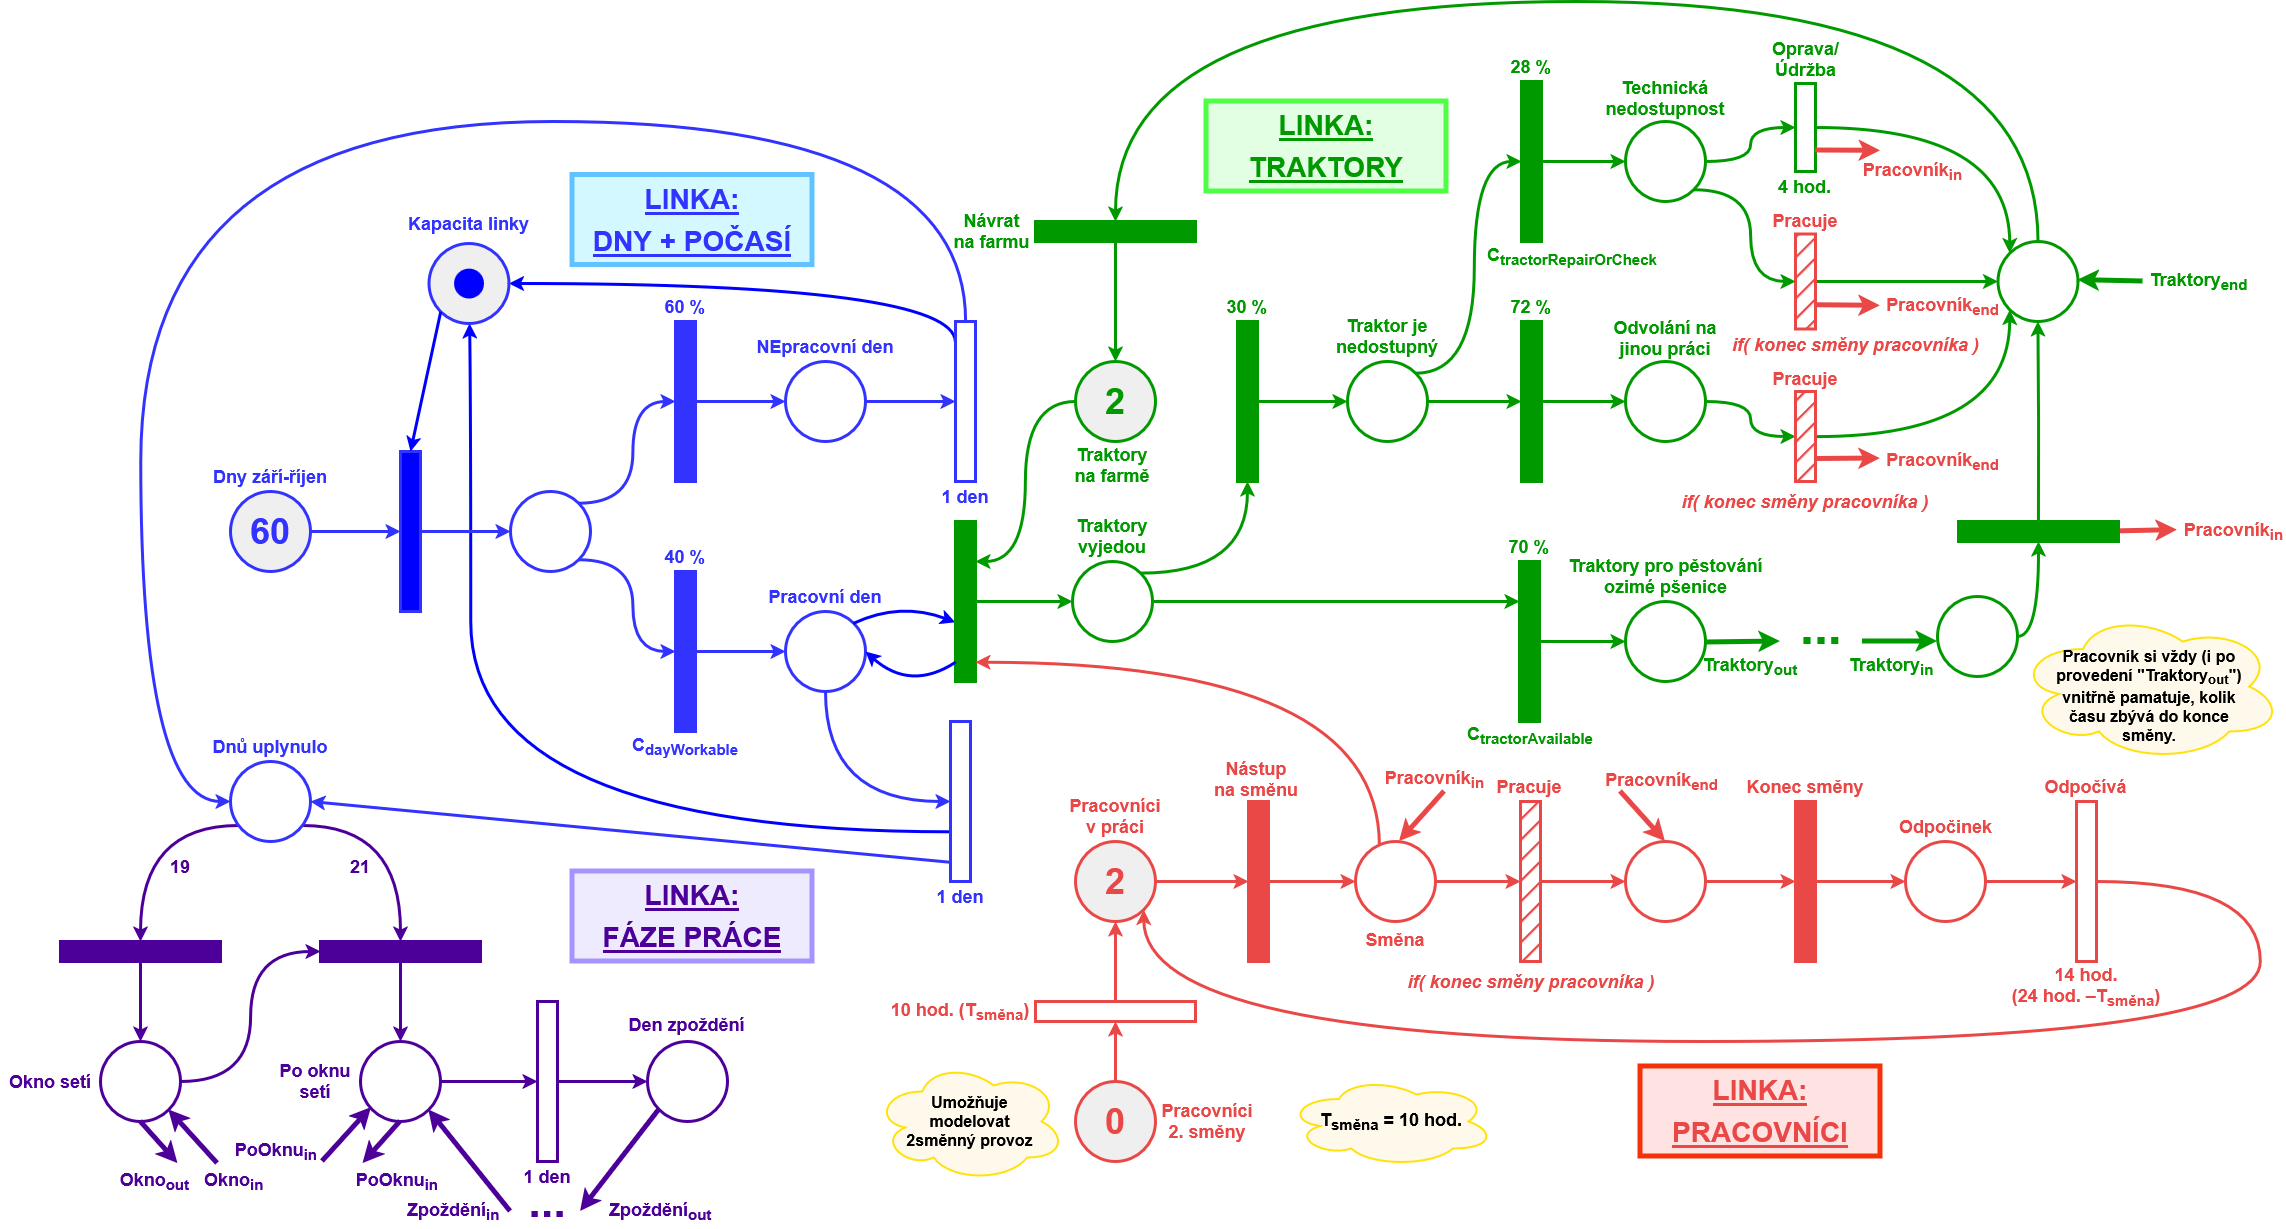
\includegraphics[width=0.9\textheight, angle=90]{Přílohy/AgroPetriNet_Resources.png}
    \caption{Modul modelující technologické linky omezených zdrojů (Dny + Počasí, Traktory, Pracovnící a Fáze práce}
    \label{fig:AgroPetriNet_Resources}
\end{figure}

\newpage

\begin{figure}[H]
    \centering
    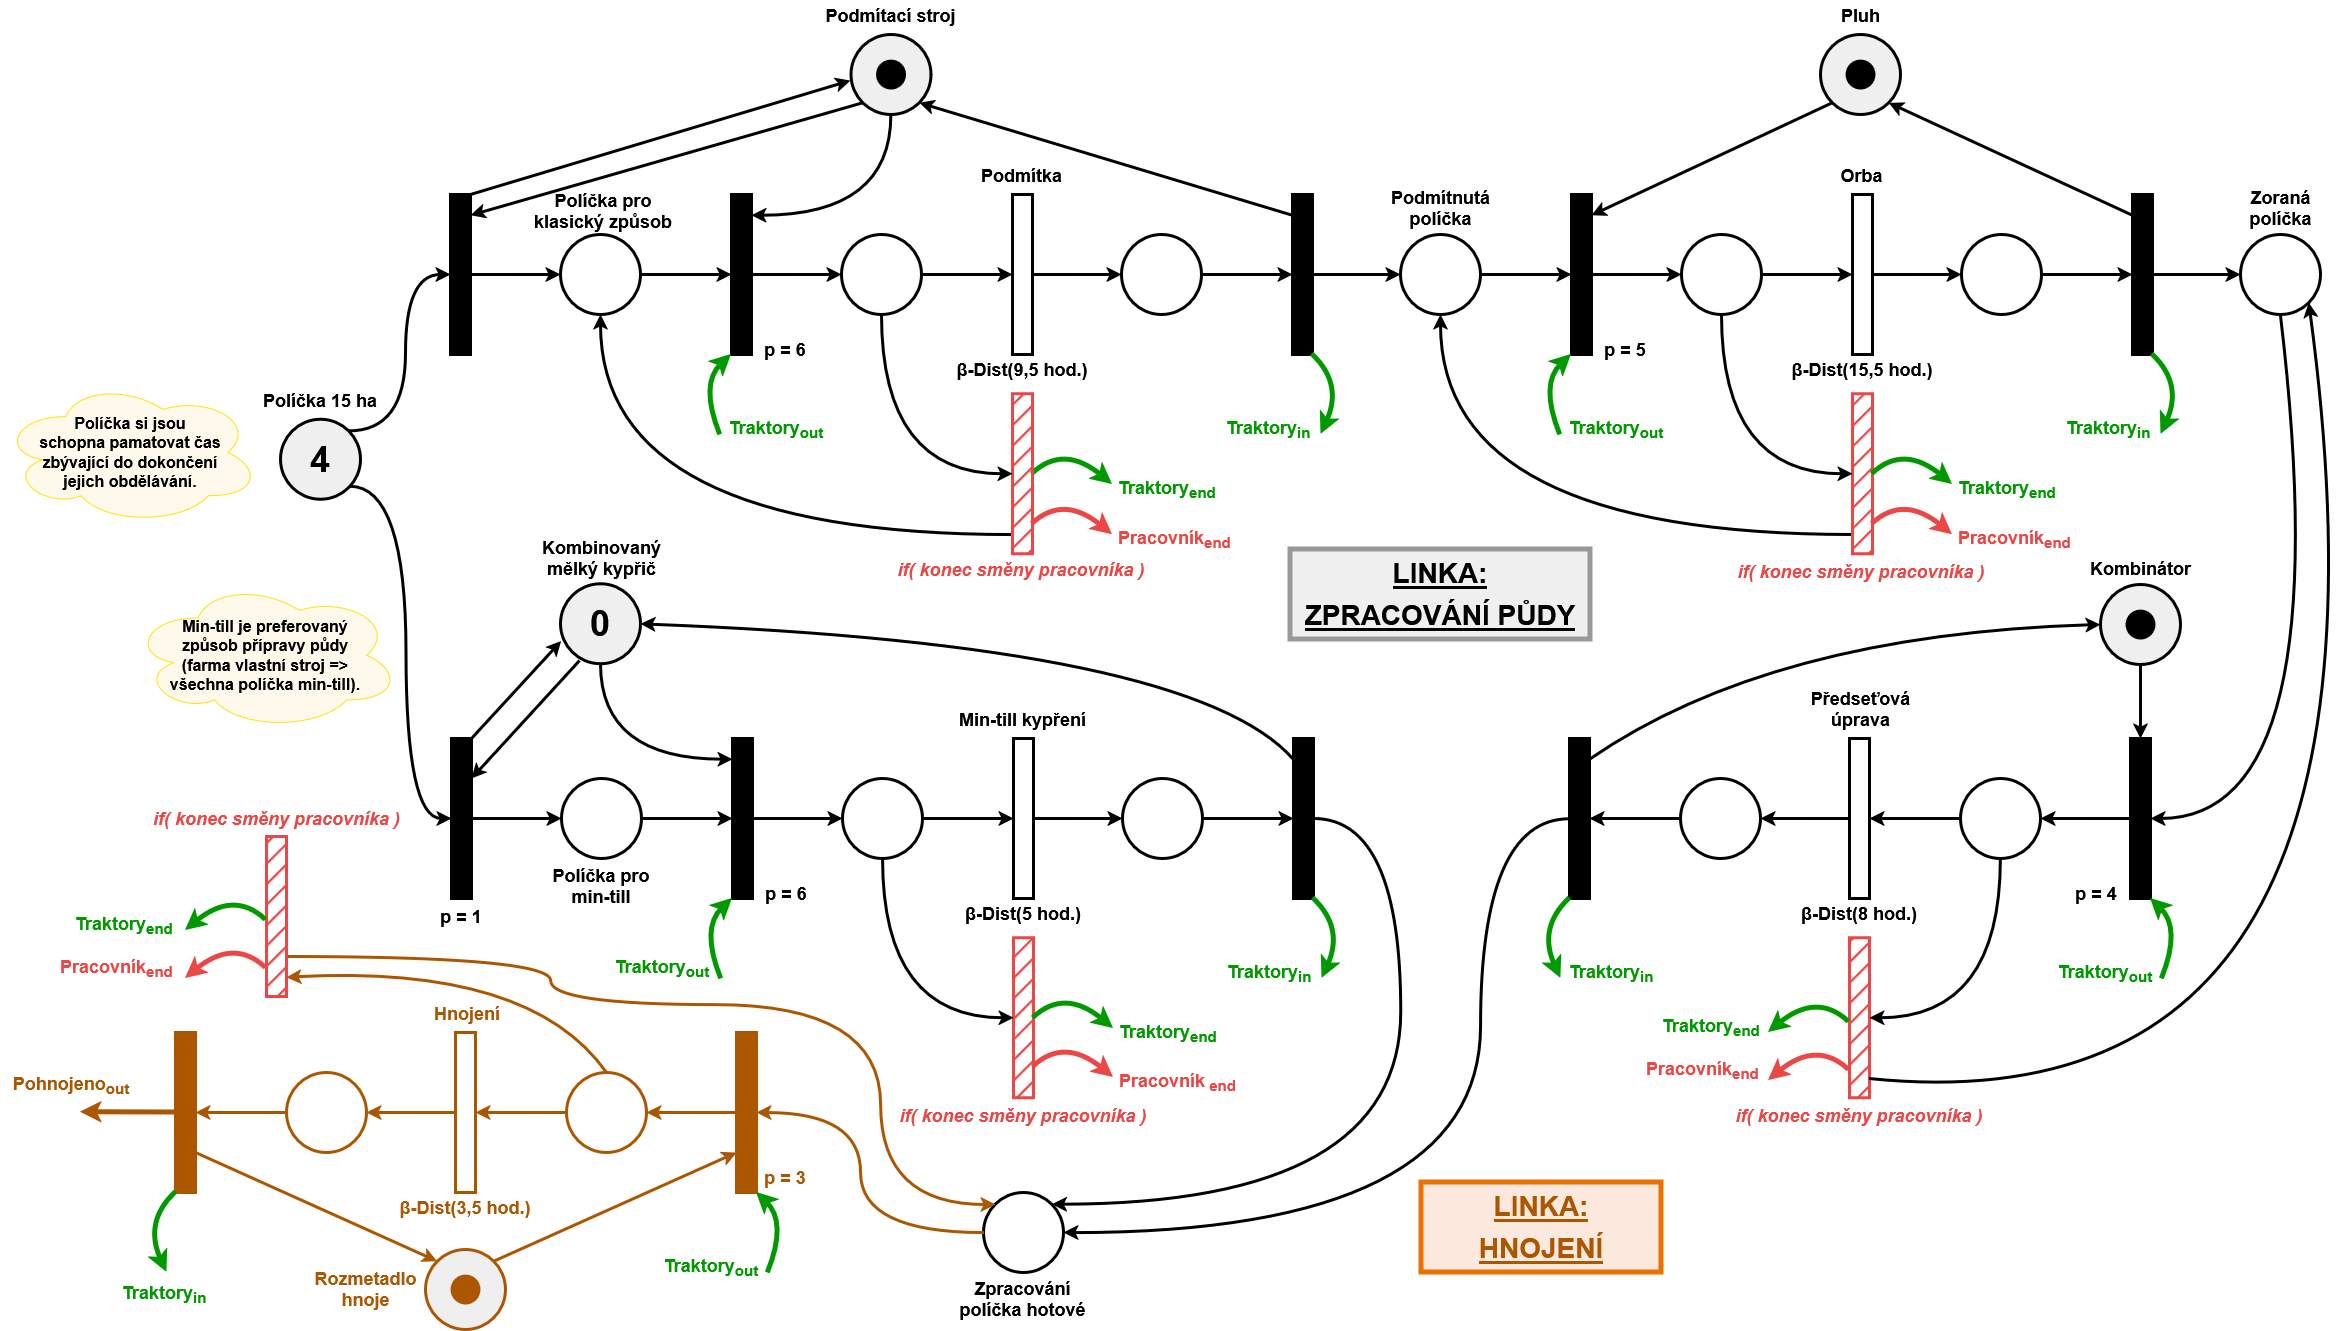
\includegraphics[width=0.95\textheight, angle=90]{Přílohy/AgroPetriNet_FieldPreparation.png}
    \caption{Modul modelující technologické linky předseťových prací}
    \label{fig:AgroPetriNet_FieldPreparation}
\end{figure}

\newpage

\begin{figure}[H]
    \centering
    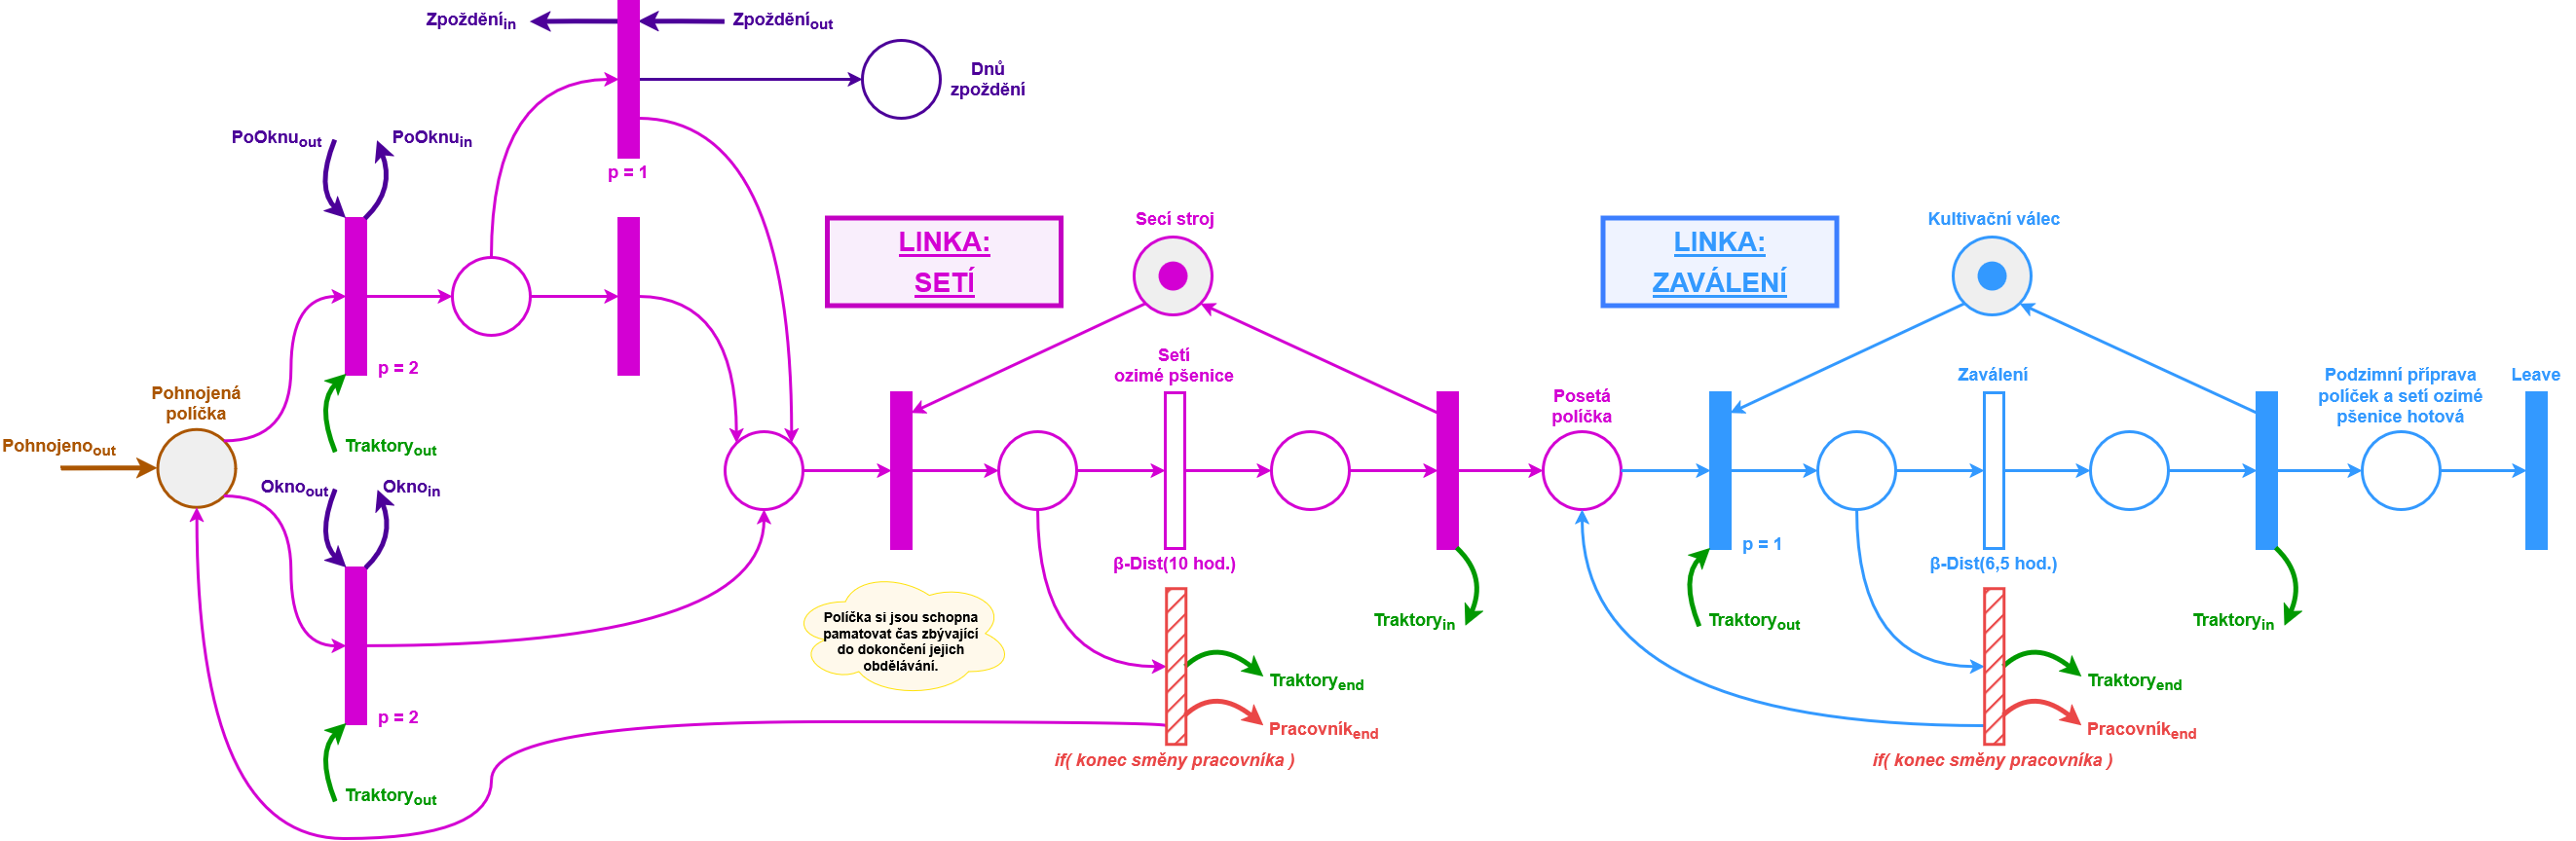
\includegraphics[width=0.95\textheight, angle=90]{Přílohy/AgroPetriNet_Cultivation.png}
    \caption{Modul modelující technologickou linku setby v~závislosti na agrotechnickém oknu a závěrečné zaválení}
    \label{fig:AgroPetriNet_Cultivation}
\end{figure}

\end{document}
